\chapter{Análisis de Resultados}
\section{Capturas del programa en ejecución}

A continuación se presenta en orden el proceso de ejecución del programa, donde primeramente se muestra el código en ejecución con un ejemplo chico y uno grande exitoso y otro grande no exitoso.\newline
\newpage

\begin{enumerate}
\item Iniciamos el programa, donde nos pide que introduzcamos una opción en el menú de inicio, la cadena que digitamos fue $"$(())()$"$. Observar la Figura 2.1.

\begin{figure}[h]
\begin{minipage}{0.3\textwidth}
    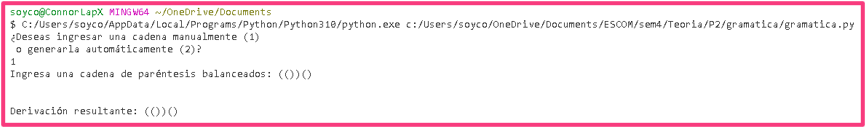
\includegraphics[width=4\linewidth]{Images/Cap1.png}
\end{minipage}
\caption{Inicio del programa en terminal.}
\label{fig:imagen}
\end{figure}
\newpage
\item Aquí se puede ver el archivo de salida de evaluacion.txt donde se pueden ver todos los pasos y reglas hechos por iteración.  Observar la Figura 2.2.\newline
\begin{figure}[h]
\begin{minipage}{0.3\textwidth}
    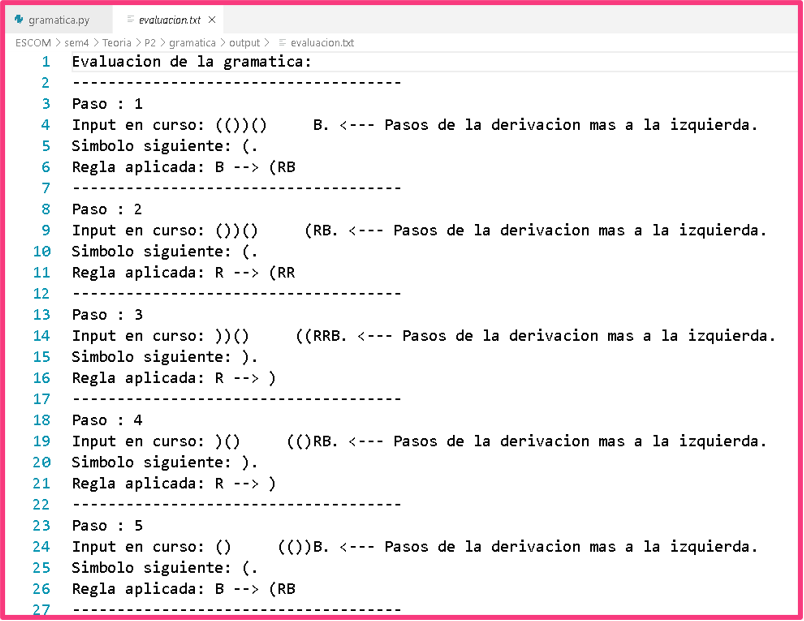
\includegraphics[width=4\linewidth]{Images/Cap2.png}
\end{minipage}
\caption{Primer parte de salida del archivo de evaluación.txt.}
\label{fig:imagen}
\end{figure}

\newpage
\item Aquí se puede ver el final del archivo de ejemplo que se ingresó como entrada, donde se pueden ver todos los pasos y reglas hechos por iteración. Observar la Figura 2.3.
\begin{figure}[h]
\begin{minipage}{0.3\textwidth}
    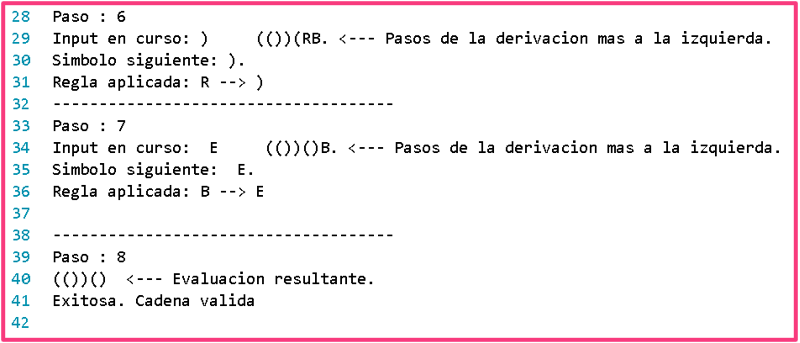
\includegraphics[width=4\linewidth]{Images/Cap3.png}
\end{minipage}
\caption{Segunda parte de salida del archivo de evaluación.txt.}
\label{fig:imagen}
\end{figure}

\newpage
\item Iniciamos nuevamente el programa, donde nos pide que introduzcamos una opción en el menú de inicio, la cadena que digitamos fue $"$)()()()()()()()()()()()()(()()()()()()()()()()()()()()(()()()()()()()()()()()()()()()()))$"$. Observar la Figura 2.4.
\begin{figure}[h]
%\begin{minipage}{0.3\textwidth}
    \begin{center}
    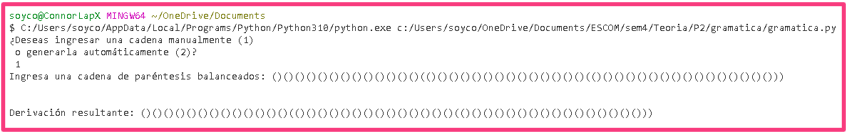
\includegraphics[width=1\linewidth]{Images/Cap4.png}
    \end{center}
%\end{minipage}
\caption{Visualización del programa en terminal.}
\label{fig:imagen}
\end{figure}

\newpage
\item Aquí se puede ver el final del archivo de ejemplo que se ingresó como entrada, donde se pueden ver todos los pasos y reglas hechos por iteración. Observar la figura 2.5.

\begin{figure}[h]
%\begin{minipage}{0.3\textwidth}
    \begin{center}
    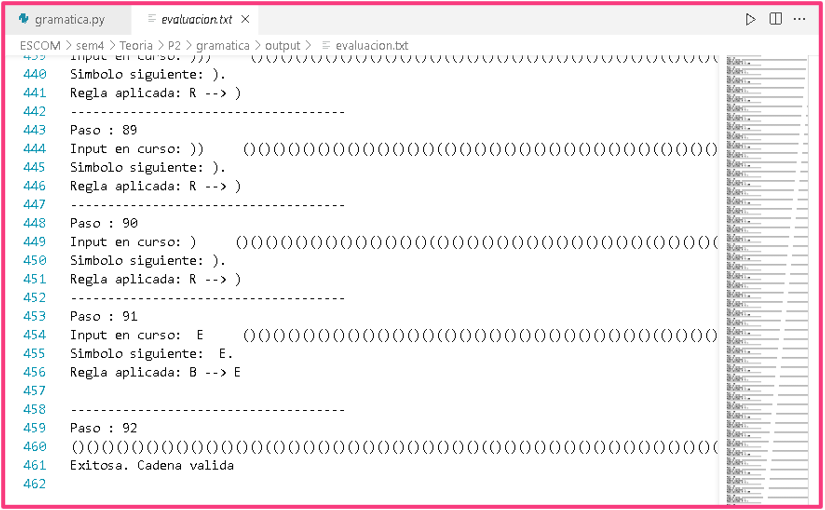
\includegraphics[width=1\linewidth]{Images/Cap5.png}
    \end{center}
%\end{minipage}
\caption{Visualización del archivo de salida evaluación.txt.}
\label{fig:imagen}
\end{figure}

\newpage
\item Iniciamos nuevamente el programa, donde nos pide que introduzcamos una opción en el menú de inicio, esta vez seleccionamos la opción aleatoria, para este ejemplo fue de tamaño 194. Observar la figura 2.6.

\begin{figure}[h]
%\begin{minipage}{0.3\textwidth}
    \begin{center}
    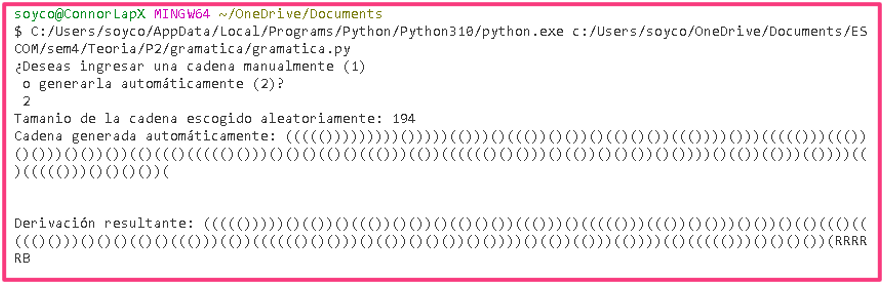
\includegraphics[width=1\linewidth]{Images/Cap6.png}
    \end{center}
%\end{minipage}
\caption{Visualización del programa en terminal.}
\label{fig:imagen}
\end{figure}
\newpage
\item Aquí se puede ver el final del archivo de ejemplo que se ingresó como entrada, donde se pueden ver todos los pasos y reglas hechos por iteración. Observar la figura 2.7.

\begin{figure}[h]
%\begin{minipage}{0.3\textwidth}
    \begin{center}
    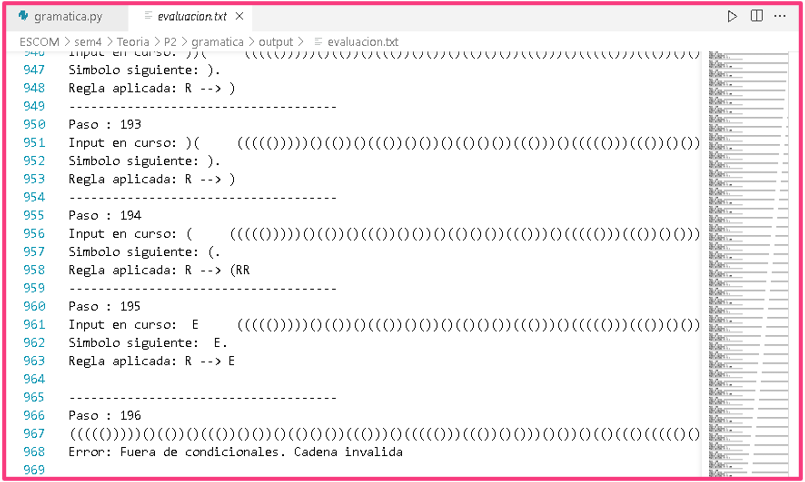
\includegraphics[width=1\linewidth]{Images/Cap7.png}
    \end{center}
%\end{minipage}
\caption{Visualización del archivo de salida evaluación.txt.}
\label{fig:imagen}
\end{figure}

\end{enumerate}